% !TeX spellcheck = en_GB

\section{Realising Temporal Bases}
\label{sec:temporal_bases}

\newcommand{\cPos}[1]{\textbf{\textcolor{DarkBlue}{#1}}}
\newcommand{\cNeg}[1]{\textbf{\textcolor{DarkRed}{#1}}}

In the previous section, we demonstrated that feed-forward networks alone are insufficient to explain the complex dynamics observed in biological systems.
However, we also demonstrated that we can realise arbitrary LTI systems of the form $\dot{\vec m}(t) = \mat A \vec m(t) + \mat B u(t)$ in recurrent \emph{linear} networks.
While we show in the next section that we can successfully solve for dynamics in networks with nonlinear neurons, our goal for now is to consider what specific temporal tuning we should \emph{optimally} realise, and how to translate this tuning into an LTI system.

As we already mentioned above, implementing an LTI system in a recurrent connection can diversify the available temporal tuning.
This in turn allows us to decode a wider range of dynamics in ensuing feed-forward sections of the network.
To maximise the set of dynamics that can be decoded, and without further knowledge about the input signals, we should optimally realise $q$ orthonormal temporal encoders $\mathfrak{e}_1(t)$, $\ldots$, $\mathfrak{b}_q(t)$ over an interval $t \in [0, \theta]$.
Orthonormality ensures that the $\mathfrak{e}_i$ are not redundant.

We first describe our overall goal more precisely, namely constructing LTI systems that approximate sliding-window spectra.
We then review common continuous and discrete bases, and discuss two methods for constructing LTI systems that generate these bases: numerically optimising an autoregressive model, and analytically solving for LTI systems generating the Legendre basis.
This latter approach yields a novel derivation of the Legendre Delay Network (LDN; \cite{voelker2018improving}) and is conceptually similar to work by \citet{gu2020hippo}.
Finally, we compare the bases generated by these systems in terms of their expressiveness.

\subsection{Computing Sliding-Window Spectra using Linear Time-Invariant Systems}
\label{sec:sliding_window_lti}

Given a function basis spanning a space such as $L^2(0, \theta)$ (cf.~\Cref{app:functional_analysis}), any function $\mathfrak{f} \in L^2(0, \theta)$ can be represented as an infinite weighted sum of basis functions $\mathfrak{b}_n$.
In the case of an orthonormal function basis (i.e., $\langle \mathfrak{b}_i, \mathfrak{b}_j \rangle = \delta_{ij}$), the corresponding weights $\chi_i$ \emph{uniquely} define each $\mathfrak{f}$ and are referred to as \emph{generalised Fourier coefficients} or the \emph{spectrum} of $\mathfrak{f}$:

\begin{definition}[{Generalised Fourier series and coefficients; cf.~\cite{young1988introduction}, Definition 4.3}]
Consider an orthonormal function basis $(\mathfrak{b}_n)_{n \in \mathbb{N}}$, where each $\mathfrak{b}_n \in L^2(0, \theta)$, as well as a function $\mathfrak{f} \in L^2(0, \theta)$. 
Then the series
\begin{align}
	\mathfrak{f} &= \sum\nolimits_{i = 0}^\infty \langle \mathfrak{f}, \mathfrak{b}_i \rangle \mathfrak{b}_i = \sum\nolimits_{i = 0}^\infty \chi_i \mathfrak{b}_i
	\label{eqn:generalised_fourier_coefficients}
\end{align}
is the generalised Fourier series of the given $\mathfrak{f}$ and $\chi_i$ are the generalised Fourier coefficients.
\end{definition}

\subsubsection{Note on using a finite number of basis functions}
In practice, it is often infeasible to realise an infinite number of basis functions.
While the $\mathfrak{b}_n$ are not necessarily ordered---any permutation $(\mathfrak{b}_{\pi(n)})_{n \in \mathbb{N}}$ still forms a valid basis---the basis functions we discuss in this section are arranged such that larger $n$ correspond to higher frequency content.
Correspondingly, only using the first $q$ basis functions results in a negligible reconstruction error if our signals are bandlimited, or, equivalently, our signals and bases are discretised appropriately (see below).

\subsubsection{Sliding-window spectrum}
Coming back to the generalised Fourier coefficients $\chi_i$, note that the inner product $\langle \mathfrak{f}, \mathfrak{b}_i \rangle$ is---time-reversal aside---merely a convolution between $\mathfrak{f}$ and $\mathfrak{b}_i$:
\begin{align*}
	\chi_i = \langle \mathfrak{f}, \mathfrak{b}_i \rangle = \int_0^\theta \!\! \mathfrak{f}(\tau) \mathfrak{b}_i(\tau) \, \mathrm{d}\tau = (\bar{\mathfrak{f}} \ast \mathfrak{b}_i)(0) \quad \quad \text{where } \bar{\mathfrak{f}}(t) \mapsto \mathfrak{f}(-t) \,.
\end{align*}
Correspondingly, if we were able to realise an LTI system that has $q$ orthonormal basis functions $\mathfrak{b}_i$ as an impulse response over a window $[0, \theta]$, then the state $\vec m(t)$ of that system would correspond to the generalised Fourier coefficients $\chi_i$ representing the past $\theta$ seconds of $u(t)$, which we denote as $u_{[t - \theta, t]} : [-\theta, 0] \longrightarrow \mathbb{R}$ with $u_{[t - \theta, t]}(\tau) \mapsto u(t + \tau)$:
\begin{align*}
	m_i(t) &= \int_0^\theta \!\! u(t - \tau) \mathfrak{b}_i(\tau) \, \mathrm{d}\tau
	        = \int_0^\theta \!\! u_{[t - \theta, t]}(-\tau) \mathfrak{b}_i(\tau) \, \mathrm{d}\tau
	        = \langle \bar u_{[t - \theta, t]}, \mathfrak{b}_i \rangle  \,.
\end{align*}
This is sometimes referred to as a \emph{sliding-window spectrum} \citep{bastiaans1985slidingwindow,denbrinler1996generalized}.%
\footnote{The cited publications use this term in the context of discrete signals, but the concept is the same.}
We illustrate this concept in \Cref{fig:lti_basis_trafo_a,fig:lti_basis_trafo_b,fig:lti_basis_trafo_c}.

\begin{figure}
	\centering
	\includegraphics{media/chapters/04_temporal_tuning/lti_basis_trafo.pdf}%
	{\phantomsubcaption\label{fig:lti_basis_trafo_a}}%
	{\phantomsubcaption\label{fig:lti_basis_trafo_b}}%
	{\phantomsubcaption\label{fig:lti_basis_trafo_c}}%
	{\phantomsubcaption\label{fig:lti_basis_trafo_d}}%
	\kern-158mm\includegraphics{media/chapters/04_temporal_tuning/lti_basis_trafo_plots.pdf}\\[0.3cm]
	\caption[Using an LTI system sliding basis transformation]{Using an LTI system $\dot{\vec m}(t) = \mat A \vec m(t) + \mat B u(t)$  as a sliding-window spectrum.
	\textbf{(A)} Any LTI system can either be implemented as using an integrator with feedback, or, as is depicted in \textbf{(B)}, by convolving $u(t)$ with the impulse response $\mathfrak{b}_i$ of each state dimension.
	\textbf{(C)} Assume that $\mathfrak{b}_i$ was a basis function over a window $[0, \theta]$.
	Then, each state dimension $m_i(t)$ is the convolution between $\mathfrak{b}_i$ and a slice of the input signal $u_{[t - \theta, t]}$.
	Correspondingly, $m_i(t)$ is the generalised Fourier coefficient $\chi_i$ describing $u_{[t - \theta, t]}$ in terms of the function basis \emph{at each point in time}.
	In other words, $\vec m(t)$ contains a compressed representation of $u_{[t - \theta, t]}$.
	\textbf{(D)} By linearly combining $\vec m(t)$ using a \enquote{decoding} matrix $\mat C$, we can approximate another LTI system, for example a delay $y(t) \approx u(t - \theta / 2)$.
	}
	\label{fig:lti_basis_trafo}
\end{figure}

\subsubsection{Transforming the sliding-window spectrum}
Another way to interpret $\vec m(t)$ is as a compressed representation of $u_{[t - \theta, t]}$.
That is, realising $q$ temporal basis functions as an LTI system continuously compresses $u_{[t - \theta, t]}$ into a $q$-dimensional vector $\vec m(t)$.
Specifically, for $q \to \infty$, and as is suggested by \cref{eqn:generalised_fourier_coefficients}, we can perfectly reconstruct $u_{[t - \theta, t]}$ from $\vec m$:
\begin{align*}
	u_{[t - \theta, t]}(-\tau) &= \sum_{i = 0}^\infty m_i \mathfrak{b}_i(\tau) = \sum_{i = 0}^\infty \langle \bar u_{[t - \theta, t]}, \mathfrak{b}_i \rangle \mathfrak{b}_i(\tau) \quad\quad \text{where } 0 \leq \tau \leq \theta \,.
\end{align*}
Similarly, we can compute $u(t)$ convolved with an arbitrary function $\mathfrak{c} : [0, \theta] \longrightarrow \mathbb{R}$ by linearly combining the entries of $\vec m(t)$.
Let $\vec{c} = (c_0, c_1, \ldots) = \langle \mathfrak{c}, \mathfrak{b}_i \rangle$ be the generalised Fourier coefficients of $\mathfrak{c}$.
Then, $\langle \vec m(t), \vec{c} \rangle = (u \ast \mathfrak{c})(t)$:
\begin{align*}
	\langle \vec m(t), \vec{c} \rangle
		&= \sum_{i = 0}^\infty m_i(t) c_i
		 = \sum_{i = 0}^\infty \langle \bar u_{[t - \theta, t]}, \mathfrak{b}_i \rangle \langle \mathfrak{c}, \mathfrak{b}_i \rangle 
		 = \sum_{i = 0}^\infty \int_0^\theta \!\! \int_0^\theta \!\!
		 	\bigl( \bar u_{[t - \theta, t]}(\tau) \mathfrak{b}_i(\tau) \bigr)
		 	\bigl( \mathfrak{c}(\tau') \mathfrak{b}_i(\tau') \bigr) \,\mathrm{d}\tau \mathrm{d}\tau' \\
		&= \int_0^\theta \!\!
			\left(\sum\nolimits_{i = 0}^\infty m_i(t) \mathfrak{b}_i(\tau) \right)
			\left(\sum\nolimits_{i = 0}^\infty c_i \mathfrak{b}_i(\tau) \right) \,\mathrm{d}{\tau}
		 = \int_0^\theta \!\! u(t - \tau) \mathfrak{c}(\tau) \,\mathrm{d}{\tau}
		 = (u \ast \mathfrak{c})(t) \,.
\end{align*}
Where the step from the first to the second line follows from $\langle \mathfrak{b}_i, \mathfrak{b}_j \rangle = \delta_{ij}$.

An example of this is illustrated in \Cref{fig:lti_basis_trafo_d}, where we decode a delay $\mathfrak{c}(t) = \delta(t - \nicefrac{\theta}2)$ by linearly combining the three state dimensions $m_i(t)$.
Since $q = 3$ is finite, we cannot use $\vec c$ as defined above, but must instead solve the least-squares problem discussed in the context of approximating dynamics in feed-forward networks (i.e., eq.~\ref{eqn:weight_optimise_currents_temporal}).

For $q \to \infty$, $\vec m(t)$ represents all information in the windowed input signal $u_{[t - \theta, t]}$.
Correspondingly, we can compute any nonlinear function over $u_{[t - \theta, t]}$ by transforming $\vec m(t)$ nonlinearly.
We could, for example, represent $\vec m$ in a neuron population and decode a function $f(\vec m)$; if we learn this decoder online, we have an \emph{adaptive filter} (cf.~\Cref{sec:adaptive_filter}).

\subsection{Continuous and Discrete Orthonormal Function Bases}
\label{sec:function_bases}

\begin{figure}
	\includegraphics{media/chapters/04_temporal_tuning/continuous_bases.pdf}%
	{\phantomsubcaption\label{fig:fourier_series}}%
	{\phantomsubcaption\label{fig:cosine_series}}%
	{\phantomsubcaption\label{fig:legendre_series}}%
	\caption[Orthonormal basis functions]{
	Orthonormal basis functions. All plots are to scale, the dotted line is zero, ticks are $0$, $\theta$.}
\end{figure}

We next review three orthonormal bases spanning $L_2(0, 1)$: the Fourier and cosine series, as well as the shifted orthonormal Legendre polynomials.

\subsubsection{Fourier and cosine series}
The most prominent function basis for temporal representations is the Fourier series. This basis is closely related to the Fourier transformation.%
\footnote{While related, the Fourier series and Fourier transformation are different concepts.
The Fourier series spans a function space over $[0, 1]$, whereas the Fourier transformation maps functions $f : \mathbb{R} \longrightarrow \mathbb{C}$ onto functions $\mathcal{F}(f) : \mathbb{C} \longrightarrow \mathbb{C}$.
Still, the generalised Fourier coefficients $\chi_i$ of a function $f$ with respect to the Fourier series can be interpreted as the real and imaginary coefficients of the Fourier transformation for specific frequencies.}

\begin{definition}[Fourier series]

The Fourier series $(f_n)_{n \in \mathbb{N}}$ over $[0, 1]$ is given as
\begin{align}
		f_0(x) &= 1 \,,&
		f_{2n + 1}(x) &= \sqrt{2}\sin\bigl(2 \pi nx\bigr) \,, &
		f_{2n} &= \sqrt{2}\cos\bigl(2 \pi nx\bigr) \,.
		\label{eqn:fourier_series}
	\end{align}
\end{definition}

\noindent The first $f_i$ are depicted in \Cref{fig:fourier_series}.
Note the sine and cosine pairs, and that each function in the Fourier series is periodic over $[0, 1]$, that is $f_n(0) = f_n(1)$.
Correspondingly, if we truncate the Fourier series to $q$ terms, we can only represent periodic functions.

An arguably simpler alternative to the Fourier series is the cosine series.
This series skips the \enquote{sine} terms of the Fourier series and increments the frequency in steps of $\pi$ instead of $2\pi$.

\begin{definition}[Cosine series]
	The cosine series $(c_n)_{n \in \mathbb{N}}$ over $[0, 1]$ is given as
	\begin{align}
	 	c_0(x) &= 1 \,, &
	 	c_n(x) &= \sqrt{2}\cos(\pi n x) \,.
	 	\label{eqn:cosine_basis}
	\end{align}
\end{definition}

\noindent Again, the first $c_i$ are depicted in \Cref{fig:cosine_series}.
Since the cosine basis is aperiodic ($f_i(0) \neq f(1)$ for odd $i$), it is better suited to representing aperiodic functions if we only have a truncated basis with $q$ terms.
Natural signals are typically aperiodic with respect to a fixed sliding window.

\subsubsection{Polynomial bases}

An alternative to trigonometric bases are polynomial bases.
%\footnote{Confusingly, the Fourier and related series are sometimes referred to as \enquote{trigonometric polynomials}.}
Examples include the Legendre, Chebyshev, Laguerre, Hermite, and Jacobi polynomials (e.g., \cite{press2007numerical}, Section~4.6.1; \cite{arfken2005mathematical}, Chapter~12).
For our purposes, the Legendre basis is most interesting.
It is aperiodic, and in contrast to the other listed polynomial bases, orthogonal with respect to a constant weighting $W(x) = 1$.

\begin{definition}[Legendre polynomials]
\label{def:legendre_polynomial}
Legendre polynomials are uniquely defined as a sequence of functions $(p_n)_{n \in \mathbb{N}}$ over $[-1, 1]$ with the following properties: \emph{(1)} $p_n$ is a polynomial of order $n$, \emph{(2)} the $p_n$ are orthogonal ($\langle p_i, p_j \rangle = 0$ exactly if $i \neq j$), and \emph{(3)} $p_n(1) = 1\,$.
\end{definition}

\subsubsection{Recurrence relation}
Starting with the base cases $p_0(x) = 1$ and $p_1(x) = x$, the Legendre polynomials $p_n(x)$ are typically defined as a recurrence relation \citep[Section~4.6.1]{press2007numerical}:
\begin{align}
	(n + 1) p_{n + 1}(x) &= (2n + 1) x p_n(x) - n p_{n - 1}(x) \,.
	\label{eqn:leg_rec}
\end{align}
%Rewriting this in terms of the polynomial coefficients $\alpha_{n, i}$ (see above) we get
%\begin{align*}
% 	(n + 1) \alpha_{n + 1, i} &= \begin{cases}
% 		\hspace{6.6em} - \, n \alpha_{n - 1, i} & \text{if } i = 0 \,, \\
% 		(2n + 1) \alpha_{n, i - 1} - n \alpha_{n - 1, i} & \text{if } i > 0 \,.
% 	\end{cases}
%\end{align*}

\subsubsection{Closed form equation}
Alternatively, the \emph{orthonormal} shifted Legendre polynomial $\tilde p_n$ over $[0, 1]$ are given in closed form as
\begin{align}
   \tilde p_n(x) &= \sqrt{2n + 1} \, (-1)^n \sum_{i = 0}^n (-1)^i \binom{n}{i} \binom{n + i}{i} x^i \,.
   	\label{eqn:legendre_basis}
\end{align}
This basis is depicted in \Cref{fig:legendre_series}. It spans $L^2(0, 1)$, just like the Fourier and cosine basis.

\subsubsection{Discrete Orthonormal Function Bases}
Continuous basis functions are useful for mathematical analysis.
However, in practice, we often divide the interval $[0, 1]$ into $N$ individual samples.
Specifically, we use such discrete bases in our numerical method for deriving $\mat A$, $\mat B$, and at the end of this chapter in \Cref{sec:applications_to_ml} when we discuss applications to machine learning.

Of course, from a mathematical perspective, the notion of \enquote{discrete function bases} is at most moderately exciting---once we discretise functions over an interval, we end up with finite-dimensional vector spaces over $\mathbb{R}^N$.
Still, there is some room for defining the concept of \enquote{discrete function bases} in relation to their continuous counterparts more rigorously.
Although our definitions are non-canonical, our notation roughly follows \citet{neuman1974discrete}.

\begin{definition}[Discrete Function Basis]
	\label{def:discrete_function_basis}
 	A \emph{discrete function basis} with an associated continuous function basis $(\mathfrak{b}_n)_{n \in \mathbb{N}}$ over $[0, 1]$ is a finite sequence of discrete basis functions $(E_n(k; N))_{n < N}$.
 	$n \in \{0, \ldots, N - 1\}$ is the basis function index, $k \in \{0, \ldots, N - 1\}$ is the sample index, and $N \geq 2$ is the number of samples.
 	The codomain of $E_n(k; N)$ is $\mathbb{R}$.
 	It must hold
 	\begin{align}
 		\lim_{N \to \infty} E_n \left( k; N \right) &= \frac{1}{\sqrt{N}} \mathfrak{b}_n\left(\frac{k}{N - 1}\right) \,, &
 		\text{and }
 		\sum_{k = 0}^{N - 1} E_i(k; N) E_j(k; N) &= \delta_{ij} \text{ if } E \text{ is orthonormal}\,.
 		\label{eqn:discrete_basis}
 	\end{align}
 	We call a matrix $\mat E \in \mathbb{R}^{q \times N}$ with $(\mat E)_{ij} = E_i(j; N)$ a \emph{basis transformation matrix}.
	In contrast to normal terminology we refer to $\mat E$ as \emph{orthonormal} if $\mat E^T \mat E = \mat I$, even if $\mat E$ is not square ($q < N$).
\end{definition}

Note that for $q = N$ an orthonormal basis transformation matrix $\mat E$ is an orthonormal basis of $\mathbb{R}^N$.
For $q < N$, the operation $\mat E \vec x$ lossily compresses $\vec x \in \mathbb{R}^N$ into a $q$-dimensional space.

\begin{figure}[t]
	\centering
	\includegraphics{media/chapters/04_temporal_tuning/discrete_basis_visualisation.pdf}%
	{\phantomsubcaption\label{fig:discrete_fourier}}%
	{\phantomsubcaption\label{fig:discrete_cosine}}%
	{\phantomsubcaption\label{fig:discrete_dlop}}%
	\caption[Visualisation of the discrete Fourier, cosine, and Legendre basis]{Visualisation of the discrete Fourier, cosine, and DLOP (Legendre) basis for $q = N = 40$.
	Each pixel is a separate sample. Red corresponds to negative values, blue to positive, grey to zero.}
\end{figure}

\subsubsection{Discrete Fourier and cosine basis}
Choosing the sample points carefully, we obtain the discrete Fourier $F_n$ and cosine bases $C_n$ used in the discrete Fourier and cosine transforms (DFT and DCT-II) and visualised in \Cref{fig:discrete_fourier,fig:discrete_cosine}:%
\footnote{
For even $N$, $F_{N - 1}$ must be rescaled to maintain orthonormality; we ignore this in our definition for terseness.
}
\begin{align}
  	F_0(k; N) &= \frac{1}{\sqrt{N}} \,, &
  	F_{2n + 1}(k; N) &= \frac{\sqrt{2}}{\sqrt{N}} \sin\left(
  		2 \pi n \frac{k + \frac{1}2}{N}\right) \,, &
  	F_{2n}(k; N) &= \frac{\sqrt{2}}{\sqrt{N}} \cos\left(
  		2 \pi n \frac{k + \frac{1}2}{N}\right) \,, \notag\\
  	C_0(k; N) &= \frac{1}{\sqrt{N}} \,, &
  	C_n(k; N) &= \frac{\sqrt{2}}{\sqrt{N}} \cos\left(\pi n \frac{k + \frac{1}2}{N}\right) \,.
  	\label{eqn:dft_dct}
\end{align}
In both cases, fast algorithms exist for computing $\mat F \vec x$ and $\mat C \vec x$ in $\mathcal{O}(N\log{N})$ instead of $\mathcal{O}(N^2)$, namely the FFT and FCT \citep[Chapter~12]{cooley1965algorithm,makhoul1980fast,press2007numerical}.

\subsubsection{Discrete Legendre Orthogonal Polynomials (DLOPs)}
A discrete version of the Legendre polynomials can be generated using the following recurrence relation (depicted in \Cref{fig:discrete_dlop}):
\begin{align*}
  	P_{0}(k; N) &= \frac{1}{\sqrt{N}} \,, \quad\quad
  	P_{1}(k; N)  = \frac{(2 k - N + 1)}{N - 1} \sqrt{\frac{3 (N - 1)}{N (N + 1)}} \,, \\
  	P_{n}(k; N) &= P_{n - 1}(k; N) \frac{(2n - 1) (N - 2k - 1)}{n (N - n)} \sqrt{\frac{\alpha_{n}(N)}{\alpha_{n - 1}(N)}}
                   - P_{n - 2}(k; N) \frac{(n - 1) (N + n - 1)}{n (N - n)} \sqrt{\frac{\alpha_{n}(N)}{\alpha_{n - 2}(N)}} \,.
\end{align*}
Where the normalisation factor $\alpha_n(N)$ is given as
\begin{align*}
 	\alpha_n(N) &= \frac{(2n + 1) (N - 1)^{(n)}}{(N + n)^{(n + 1)}} & \text{where } k^{(i)} &= \prod_{j = 0}^{i - 1} (k - j) = \frac{k!}{(k - i)!} \text{ is the $i$th fading factorial of $k$.}
\end{align*}
These \enquote{Discrete Legendre Orthogonal Polynomials} (DLOPs) have first been proposed by \citet{neuman1974discrete}.
Our modified recurrence relation above is numerically stable and directly produces an orthonormal basis. We provide a more detailed discussion in \citet{stockel2021discrete}.

\subsection{Numerically Solving for Linear Time Invariant Systems}
\label{sec:lti_autoregression}

Our next goal is to construct LTI systems $\dot{\vec m}(t) = \mat A \vec m(t) + \mat B u(t)$ that generate the above bases using only $q$ state dimensions.
To this end, we first describe a numerical method, and then, in the next subsection, analytically solve for $\mat A$, $\mat B$ in the specific case of the Legendre basis.

\subsubsection{Auto-regressive system identification}
Consider an orthonormal basis transformation matrix $\mat M \in \mathbb{R}^{q \times N}$. The $i$th column (with $i \in \{1, \ldots, N\}$) of $\mat M$, here denoted as $\vec m_i$, is a $q$-dimensional vector describing the impulse response of the desired system at $t = \Delta t i$, where $\Delta t = \theta / N$.
If this state evolution is indeed the result of a time-invariant linear process, then we have
\begin{align*}
	\vec m_0 &= \mat{\tilde B} \,, &
	\vec m_{i + 1} &= \vec m_{i} + \Delta t \mat{\tilde A} \vec m_i
	\quad \Leftrightarrow \quad
	\mat{\tilde A} \vec m_{i} = \frac{\vec m_{i + 1} - \vec m_i}{\Delta t} \quad \text{for all} \quad 1 \leq i < N \,,
\end{align*}
where $\mat{\tilde B}$ describes the influence of the initial impulse on the state, and $\mat{\tilde A}$ is the state-transition matrix.
Finding a $\mat{\tilde A}$ with this property can be written as a linear least-squares problem:
\begin{align}
	\mat{\tilde A} = \arg\min_{\mat{\tilde A}} \sum_{i = 1}^{N - 1} \left\| \mat{\tilde A} \vec m_i - \frac{\vec m_{i + 1} - \vec m_i}{\Delta t} \right\|_\mathrm{F}^2 \,.
	\label{eqn:construct_lti_lstsq}
\end{align}
This is a standard auto-regressive linear model \citep[cf.][Chapter~8]{verhaegen2007filtering}; of course, we could use the derivative of a continuous basis instead of the difference quotient.
Assuming that $\mat{\tilde A}$ and $\mat{\tilde B}$ are the result of discretising the LTI system with a zero-order hold assumption \citep[e.g.,][Section~9.8]{brogan1991modern}, we obtain a continuous system $\mat A$, $\mat B$ as follows:
\begin{align}
 	\mat A &= \frac{1}{\Delta t} \log\bigl(\mat I  + \Delta t \mat{\tilde A}\bigr) \,, &
 	\mat B &= \sqrt{N} \mat{\tilde B} \,,
 	\label{eqn:lti_inverse_discretisation}
\end{align}
where \enquote{$\log$} is the matrix logarithm, the inverse operation of taking the matrix exponential.
%Scaling $\mat{\tilde B}$ by $\sqrt{N}$ is necessary to obtain orthonormal basis functions.

\begin{figure}
	\centering
	\includegraphics{media/chapters/04_temporal_tuning/construct_lti.pdf}
	\caption[LTI systems generating the Fourier, cosine and Legendre basis]{LTI systems generating the Fourier, cosine and Legendre basis.
	Constructed using \cref{eqn:construct_lti_lstsq,eqn:lti_inverse_discretisation} and $N = 1000$ samples.
	\emph{Top:} NRMSE $E$ over $[0, \theta]$ between the LTI impulse response and the reference basis functions (excluding the constant $\mathfrak{b}_0$). Black cross is the mean, error bars the minimum and maximum error over $q - 1$ basis functions.
	\emph{Bottom:} First six dimensions of the reconstructed LTI system impulse response for $q = 11$ basis functions (cf.~above arrow); dotted line is the reference.
	\textbf{(A)} The Fourier basis can be constructed well by an LTI system for odd $q$ (mean $E < 10^{-2}$).
	\textbf{(B)} The cosine basis can only be realised as an LTI system with relatively large errors (mean $E > 10^{-1}$). Adding more basis functions reduces the error for earlier basis functions.
	\textbf{(C)} The Legendre basis can be realised well with small errors for all $q$ (mean $E < 2^{-2}$).
	}
	\label{fig:construct_lti}
\end{figure}

\Cref{fig:construct_lti} depicts the impulse responses of LTI systems constructed in this manner.
The method works well for the Fourier and the Legendre basis, but results in relatively large errors in the case of the cosine basis; particularly for later basis functions.
Since the Fourier system consists of $(q - 1) / 2$ harmonic oscillators requiring two state-dimensions each, $q$ must be odd.

Rather unsurprisingly, the impulse response of the generated LTI systems continues past the time-window $\theta$.
In the case of the Fourier and cosine basis, the oscillation just continues, whereas the Legendre system diverges.
To prevent this, we need to modify the system to rapidly decay to zero, preferably \emph{exactly} at time $\theta$.

\begin{figure}
	\centering
	\includegraphics{media/chapters/04_temporal_tuning/construct_lti_window.pdf}
	\caption[Windowed LTI systems generating the Fourier, cosine and Legendre basis]{
	Windowed LTI systems generating the Fourier, cosine and Legendre basis.
	Same experiment as in \Cref{fig:construct_lti_window}, but the target functions are multiplied with a linear window over $[0, \theta]$
	}
	\label{fig:construct_lti_window}
\end{figure}

\subsubsection{Window functions}
One possible solution is to multiply the desired basis with a window function $w(t) \in [0, 1]$, that is, $\mathfrak{b}'_i(t) = w(t) \mathfrak{b}_i(t)$ for $t \in [0, \theta]$.
Unfortunately, the resulting basis is no longer orthnormal, and decoding information in regions with small $w(t)$ is more difficult.

\Cref{fig:construct_lti_window} depicts results for a one-sided Bartlett window $w(t) = 1 - x \theta^{-1}$ \citep[cf.][Section~7.5]{oppenheim2009discretetime}.
Again, we are able to realise the desired dynamics well for the Fourier and Legendre basis, albeit with a large increase in error due to having to decode the window dynamics.
Furthermore, this method does not work particularly well for the cosine basis.
Although the final system is stable, we can still observe substantial oscillations for $t > \theta$.

\subsubsection{Establishing a rectangle window through \enquote{information erasure}}
Optimally, we would like to realise a rectangle window.
That is, the impulse response of our system should exactly trace out $\mathfrak{b}_i(t)$ for $t \in [0, \theta]$, and then, at $t = \theta$, drop to zero.
Phrasing this more colloquially, we must ensure that input older than $\theta$ seconds (or, in the discrete case, $N$ samples) is \enquote{forgotten}.

Accomplishing this is indeed possible, and the fact that we are realising a function basis is key.
Remember from \Cref{sec:sliding_window_lti} that we can decode a delayed version of the input signal $u(t - \theta')$ from the system state $\vec m(t)$.
We can furthermore compute the specific contribution $\vec m'(t)$ of $u(t - \theta)$ to $\vec m(t)$.
Subtracting $\vec m'(t)$ from $\vec m(t)$ effectively \enquote{erases} any information about $u(t - \theta)$ from the state vector, resulting in a finite impulse response.

We discuss this more thoroughly for continuous bases in the next subsection.
For now, in the discrete case, assume that the impulse response of the discrete LTI system $\mat{\tilde A}$, $\mat{\tilde B}$ perfectly reconstructs the basis transformation matrix $\mat E \in \mathbb{R}^{q \times N}$.
We can then reconstruct the input sample $u_{t - N + 1}$ from $\vec m_t$ using the Moore-Penrose pseudo-inverse $\mat E^+$:
\begin{align*}
 	u_{t - N + 1} &= (\mat E^+)_{N} \vec m_t \,, & \text{where } \mat E^+ = (\mat E^T \mat E)^{-1} \mat E^T\,.
\end{align*}
Let \enquote{$\odot$} denote the outer product.
The contribution of $u_{t - N + 1}$ to the state $\vec m_t$ is then given as
\begin{align*}
 	\vec m'_t &= ( \mat E^T)_N u_{t - N + 1} = ( \mat E^T)_N \odot (\mat E^+)_N\vec m_t \,.
\end{align*}
Sequentially interleaving an \enquote{update} and an \enquote{erasure} step we obtain
\begin{align}
 	\vec m_t &\gets \mat{\tilde A} \vec m_{t - 1} + \mat{\tilde B} u_t \,, \tag{Update}\\
 	\vec m_t &\gets \vec m_t - \vec m'_t = ( \mat I - ( \mat E^T )_N \odot (\mat E^+)_N ) \vec m_t \,. & \tag{Erasure}\\[-0.5em]
 	\cline{1-2}
 	\vec m_t &\gets
 		(\mat I - ( \mat E^T )_N \odot (\mat E^+)_N ) \mat{\tilde A} \vec m_t
 		+ (\mat I - ( \mat E^T )_N \odot (\mat E^+ )_N ) \mat{\tilde B} u_t
 		=   \mat{{\tilde A}'} \vec m_{t - 1} + \mat{{\tilde B}'} u_t  \,.
	\label{eqn:information_erasure_discrete}
\end{align}
Applying the inverse discretisation from \cref{eqn:lti_inverse_discretisation} to $\mat{\tilde A}'$, $\mat{\tilde B}'$ results in a dampened, continuous LTI system.
Importantly, this is only an optimal solution if $\mat{\tilde A}$ and $\mat{\tilde B}$ perfectly reconstruct the discrete function basis.
Furthermore, this technique cannot work with periodic bases (i.e., the Fourier basis), since there is technically no difference between decoding $u(t)$ and $u(t - \theta)$.

\begin{figure}
	\centering
	\includegraphics{media/chapters/04_temporal_tuning/construct_lti_erasure.pdf}%
	{\phantomsubcaption\label{fig:construct_lti_erasure_a}}%
	{\phantomsubcaption\label{fig:construct_lti_erasure_b}}%
	{\phantomsubcaption\label{fig:construct_lti_erasure_c}}
	\caption[Effect of the \enquote{information erasure} technique on LTI systems generating function bases]{
	Effect of the \enquote{information erasure} technique (eq.~\ref{eqn:information_erasure_discrete}) on LTI systems generating function bases.
	\emph{Top, bottom:} Same analysis as in \Cref{fig:construct_lti_window}.
	\emph{Middle:} RMS $E'$ of the response over $[\theta, 2\theta]$.
	Blue cross is the mean, bars are the minimum and maximum over the last $q - 1$ basis functions.
	\textbf{(A)}~We use a modified Fourier basis with halved frequency (see text).
	Reconstruction errors $E$ are small compared to the other bases; the basis quickly decays to zero.
	\textbf{(B)}~The dampened LTI system generating the cosine basis is stable, but possesses substantial oscillations for $t > \theta$.
	\textbf{(C)}~Dampening introduces substantial ringing artefacts in the Legendre basis, but the impulse response quickly decays to zero.
	}
	\label{fig:construct_lti_erasure}
\end{figure}

\begin{figure}
	\centering
	\includegraphics{media/chapters/04_temporal_tuning/construct_lti_feedback_matrices.pdf}
	\caption[Feedback matrices generating LTI systems and their eigenvalues]{Feedback matrices generating LTI systems and their eigenvalues.
	\emph{Top:} Visualisation of the feedback matrices $\mat A$ for $q = 11$, red corresponds to negative, blue to positive values, grey is zero. \emph{Bottom:} Real and imaginary components of the corresponding eigenvalues. \textbf{(A, B)} With and without information erasure.
	Note the regular structure of $\mat A$. Information erasure ensures stability, i.e., negative $\mathrm{Re}(\lambda_i)$.
	The eigenvalues of the dampend Fourier and Legendre systems are qualitatively similar.
	}
	\label{fig:construct_lti_feedback_matrices}
\end{figure}

\Cref{fig:construct_lti_erasure} depicts the effects of this \enquote{information erasure} procedure on the LTI systems generating a modified Fourier, cosine and Legendre bases.
Specifically, we slow the oscillations of the Fourier basis by $10\%$, making the basis aperiodic and compatible with information erasure.
This comes at the cost of the new basis being non-orthonormal, and thus information-theoretically suboptimal.
For both this modified Fourier and Legendre basis, our method indeed approximates a rectangle window, yet introduces ringing artefacts over $[0, \theta]$.
The method stabilises the cosine basis, but there are still residual oscillations for $t > \theta$---this is likely because the cosine basis is not realised well by our LTI system (see previous experiments).

The feedback matrices $\mat A$ are depicted in \Cref{fig:construct_lti_feedback_matrices}.
Their regular $\mat A$ suggests that we might be able to construct these matrices analytically; for example, the Fourier system feedback matrices merely construct a set of harmonic oscillators.
As we show next, the Legendre system can similarly be derived from first principles.

\subsection{Closed-Form Solution for the Legendre Basis}
\label{sec:ldn_derivation}

While our numerical method for approximating function basis generating LTI systems works amiably well, we can, in some cases, analytically determine LTI systems that generates bases over an approximated rectangle window.
For example, as we show next, we can analytically construct an LTI system ${\mat A}$, ${\mat B}$ that \emph{exactly} traces out the Legendre polynomials.
In particular, we use a continuous variant of our above information erasure technique to construct a dampening term $\mat \Gamma$ that limits the impulse response of the system to $[0, \theta]$.
Subtracting $\mat \Gamma$ from $\mat A$ we obtain a rescaled version of the LTI system underlying the Legendre Delay Network (LDN; \cite{voelker2018improving}).
This idea is similar to \citet{gu2020hippo} and can, as we discuss in more detail in \citet{stockel2021constructing}, be applied to arbitrary polynomial bases.

%\begin{figure}
%	\small
%	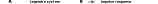
\includegraphics{media/chapters/04_temporal_tuning/leg_sys_example_header.pdf}
%	\begin{minipage}[b]{0.5\textwidth}
%	\begin{align*}
%		\hspace*{0.5em}{\mat A} &= \begin{pmatrix}
%			      0    &	      0    &	      0    &	      0    &	      0    &	      0    \\
%			\cPos{2}   &	      0    &	      0    &	      0    &	      0    &	      0    \\
%			      0    &	\cPos{6}   &	      0    &	      0    &	      0    &	      0    \\
%			\cPos{2}   &	      0    &	\cPos{10}  &	      0    &	      0    &	      0    \\
%			      0    &	\cPos{6}   &	      0    &	\cPos{14}  &	      0    &	      0    \\
%			\cPos{2}   &	      0    &	\cPos{10}  &	      0    &	\cPos{18}  &	      0
%		\end{pmatrix} &
%		{\mat B} &= \begin{pmatrix}
%			\cPos{1}   \\
%			\cNeg{-1}  \\
%			\cPos{1}   \\
%			\cNeg{-1}  \\
%			\cPos{1}   \\
%			\cNeg{-1}
%		\end{pmatrix}\\[0.475em]
%	\end{align*}
%	\end{minipage}%
%	\includegraphics{media/chapters/04_temporal_tuning/leg_sys_example.pdf}
%	\caption[Example of the Legendre system and the corresponding impulse response]{Example of the Legendre system for $q = 6$ and $\theta = 1$ \textbf{(A)} and the corresponding impulse response \textbf{(B)}. The impulse response of the system (coloured lines) perfectly traces out the first six shifted Legendre polynomials $\tilde P_i(\theta)$ normalised to $\tilde P_i(1) = 1$ (black dotted lines).}
%	\label{fig:leg_sys_example}
%\end{figure}

\begin{restatable}{lemma}{LemLegSys}
The impulse response of the linear time-invariant system $\theta \dot{\vec m}(t) = {\mat A} \vec m(t) + {\mat B} u(t)$ with $\vec m \in \mathbb{R}^q$, ${\mat A} \in \mathbb{R}^{q \times q}$ and ${\mat B} \in \mathbb{R}^{q \times 1}$
\begin{align*}
	\begin{aligned}
	\big({\mat A}\big)_{ij} &= (4j - 2) \begin{cases}
			0 & \text{if } i \leq j \text{ or } i + j \text{ is even} \,, \\
			4j - 2 & \text{if } i > j \text{ and } i + j \text{ is odd} \,,
		\end{cases} &
	\big({\mat B}\big)_i &= (-1)^{i + 1} \,,
	\end{aligned}
\end{align*}
are the first $q$ shifted Legendre polynomials $\tilde P_n(t \theta^{-1})$ scaled to $\tilde P_n(1) = 1$ over $t \in [0, \theta]$.
\label{lem:leg_sys}
\end{restatable}
\noindent We provide a proof of this lemma in \Cref{app:leg_sys_proof}; see \Cref{fig:ldn_example_a} for an example.
As before, we now need to limit the impulse response of this system to a rectangle window $[0, \theta]$.
This would be trivial if we had access to a delayed version $u(t - \theta)$ of the signal:
\begin{restatable}{lemma}{LemRectangleWindow}
\label{lem:rectangle_window}
Let $\mat A$, $\mat B$ describe an LTI system and let $u(t)$ be some input signal.
The impulse response of the following modified system is unchanged compared to the original LTI system for $0 \leq t < \theta$ but zero for all $t \geq \theta$%
\begin{align*}
	\dot{\vec m}(t) &= \mat A \vec m(t) + \mat B u(t) - \vec e(\theta) u(t - \theta) \,, & \text{where } \vec e(\theta) = \exp(\mat A \theta) \mat B \,.
\end{align*}
\end{restatable}

Of course, we usually do not access to the delayed input signal $u(t - \theta)$.
However, as we discussed in \Cref{sec:sliding_window_lti,sec:lti_autoregression}, we can decode an approximate $u(t - \theta')$ from the state $\vec m(t)$ using a delay decoder $\vec d(\theta')$.
Below, we define the term \enquote{delay decoder} more precisely for input signals $\hat u(t - \theta)$ that are expressible using a $q$ basis functions.

\begin{definition}[Delay decoder]
\label{def:delay_decoder}
Let $\hat u : [0, \theta] \longrightarrow \mathbb{R}$ expressible as a linear combination of $q$ basis functions $\mathfrak{b}_n : [0, \theta] \longrightarrow \mathbb{R}$ with generalised Fourier coefficients $\chi_i$.
Let $\vec m(t)$ be the state of a $q$-dimensional system with impulse responses $\mathfrak{b}_n$ and input $\hat u$, i.e.,
\begin{align*}
	m_i(t)
		&= \int_{0}^t \mathfrak{b}_i(\tau) \hat u(t - \tau) \,\mathrm{d}\tau
		 = \int_{0}^t \mathfrak{b}_i(\tau) \sum_{j = 0}^{q - 1} \chi_j \mathfrak{b}_j(t - \tau )\,\mathrm{d}\tau \,.
\end{align*}
Then $\vec d(\theta') = (d_0(\theta'), \ldots, d_{q - 1}(\theta'))$ is called a \emph{delay decoder} if
\begin{align}
	\begin{aligned}
	\hat u(\theta - \theta')
		 = \sum_{j = 0}^{q - 1} \chi_j \mathfrak{b}_j(\theta - \theta')
		 = \big\langle \vec d(\theta'), \vec m(\theta) \big\rangle
		 = \sum_{i = 0}^{q - 1} d_n(\theta') \int_{0}^\theta \mathfrak{b}_i(\tau) \sum_{i = 0}^{q - 1} \chi_j \mathfrak{b}_j(\theta - \tau )\,\mathrm{d}\tau \,.
	\end{aligned}
	\label{eqn:delay_decoder}
\end{align}
\end{definition}

\begin{restatable}{lemma}{LemLegendreDelayDecoder}%
	\label{lem:legendre_delay_decoder}%
	For the shifted Legendre polynomials $\tilde P_i(t \theta^{-1})$ with $\tilde P_i(1) = 1$, the delay decoder is
	\begin{align*}
		d_i(\theta') = \frac{2i + 1}{\theta} \tilde P_i(\theta' \theta^{-1}) \,.
	\end{align*}
\end{restatable}
\noindent This follows from the orthogonality of $\tilde P_i(t)$. We provide a proof in \Cref{app:legendre_delay_decoder_proof}.

\begin{figure}
	\centering
	\includegraphics{media/chapters/04_temporal_tuning/ldn_example.pdf}%
	{\phantomsubcaption\label{fig:ldn_example_a}}%
	{\phantomsubcaption\label{fig:ldn_example_b}}%
	\caption[Feedback matrices and impulse responses of the Legendre system]{Feedback matrices and impulse responses of the Legendre system.
	\emph{Left:} The feedback matrix $\mat A$ of the corresponding system for $q = 6$ and $\theta = \SI{1}{\second}$. \emph{Right:} The corresponding impulse response.
	\textbf{(A)} The undampened Legendre system as described in \Cref{lem:leg_sys}.
	\textbf{(B)} The Legendre system with approximate rectangle window (cf.~\Cref{eqn:ldn_system}).¸
	}
	\label{fig:ldn_example}
\end{figure}

Given the concept of a \enquote{delay decoder} we can construct an approximate version of the windowed LTI system in \cref{lem:rectangle_window} that reconstructs $u(t - \theta)$ from the system state $\vec m(t)$
\begin{align}
	\frac{\mathrm{d}}{\mathrm{d}t} \vec m(t)
		&= \mat A \vec m(t) + \mat B u(t) - \vec e(\theta) \langle \vec d(\theta), \vec m(t) \rangle
		 = (\mat A - \mat \Gamma) \vec m(t) + \mat B u(t)
	\label{eqn:information_erasure_approx} \,,
\end{align}
where the dampening term $\mat \Gamma = \vec e(\theta) \odot \vec d(\theta)$ is the \emph{delay re-encoder}.
For the shifted Legendre polynomials $\tilde P_i(t \theta^{-1})$ with $\tilde P_i(1) = 1$ the resulting delay re-encoder is simply given as
\begin{align}
	\big( \mat{\Gamma} \big)_{ij} &= e_i(\theta) d_j(\theta) = \frac{2j + 1}{\theta} \tilde P_{i - 1}(\theta \theta^{-1}) \tilde P_{j - 1}(\theta \theta^{-1}) = \frac{2j + 1}{\theta} \,.
	\label{eqn:legendre_delay_reencoder}
\end{align}
Correspondingly, the feedback matrix $\mat A'$ of the LTI system generating the Legendre polynomials with approximated rectangle window is given as
\begin{align}
	\begin{aligned}
	\big( \mat A' \big)_{ij} &= (2j - 1) \begin{cases}
		-1 & \text{if } i \leq j \text{ or } i + j \text{ is even} \,, \\
		 1 & \text{if } i > j \text{ and } i + j \text{ is odd} \,,\\
	\end{cases} &
	\big( \mat B' \big)_i &= (-1)^{i + 1} \,.
	\end{aligned}
	\label{eqn:ldn_system}
\end{align}
The impulse response for $q = 6$ of this system is depicted in \Cref{fig:ldn_example_b}.

If we divide each state dimension by $(2 i + 1)$, we obtain exactly the same system as the one described by \citet[Section 6.3.1, pp.~133-135]{voelker2019} in the context of the Legendre delay network.
The LDN system has been derived from the Padé approximants of a Laplace domain delay $e^{-\theta s}$ and a subsequent conditioning coordinate transformation \citep{voelker2018improving}.
%\Citet{voelker2019} points out that the impulse response of the linear time-invariant (LTI) system underlying the delay network traces out the shifted Legendre polynomials.
From this perspective, the similarity of the impulse response to the Legendre polynomials is rather coincidental; our derivation strengthens the connection between the Legendre polynomials and the LDN.


\subsection{Decoding Delays as a Benchmark for Temporal Bases}
\label{sec:comparing_temporal_bases}

In theory, the different continuous and discrete function bases discussed in \Cref{sec:function_bases} possess the same representational power.
The continuous bases span the function space $L^2(0, 1)$, and the discrete bases span the $N$-dimensional vector space~$\mathbb{R}^N$.
However, we expect to see differences in how well we can decode functions as soon as we truncate the bases to $q$ terms, and even more so when generating the bases as the impulse response of an LTI system of order $q$.

One way to \enquote{benchmark} such non-ideal temporal bases is to characterise in how far we can decode delayed versions of the input signal $u(t)$ from the generalised Fourier coefficients $\vec m(t)$ \citep[cf.][]{voelker2018improving}.
This is a reasonable benchmark, since performing well in this task has implications beyond just computing delays. 
Remember that a convolution of $u(t)$ with some function $\mathfrak{c}(t) : [0, \theta] \longrightarrow \mathbb{R}$ is a weighted integral over delayed~$u(t)$:
\begin{align*}
	(u \ast \mathfrak{c})(t)
		&= \int_{0}^\theta \!\! u(t - \theta') \mathfrak{c}(\theta') \, \mathrm{d}\theta'
		 = \int_{0}^\theta \!\! \langle \vec m(t), \vec d_{\theta'} \rangle \mathfrak{c}(\theta') \, \mathrm{d}\theta'
		 = \langle \vec m(t), \vec c \rangle \,,
\end{align*}
where the vector $\vec c$ is the \enquote{filter decoder} mentioned in \Cref{sec:sliding_window_lti}.
Hence, being able to decode delays well implies that we can approximate any linear filter $\mathfrak{c}$ with a small error.

\subsubsection{Comparing windowed LTI systems to a low-pass filter basis}

\begin{figure}[t]
	\centering
	\includegraphics{media/chapters/04_temporal_tuning/delay_analysis_example.pdf}%
	{\phantomsubcaption\label{fig:delay_analysis_example_a}}%
	{\phantomsubcaption\label{fig:delay_analysis_example_b}}%
	{\phantomsubcaption\label{fig:delay_analysis_example_c}}%
	{\phantomsubcaption\label{fig:delay_analysis_example_d}}%
	\caption[Computing delays as a function basis benchmark]{Computing delays as a function basis benchmark.
	\emph{Top:} Six state dimensions $\vec m(t)$ of the underlying LTI system (order $q = 11$) for an input $u(t)$.
	\emph{Bottom}: Input $u(t)$ (dashed black line), and delayed versions decoded from $\vec m(t)$ (coloured lines).
	Depicted error $E$ is the mean NRMSE between the ground-truth $u(t - \theta')$ (assuming $u(t) = 0$ for $t < 0$) and the decoded delays.
	\textbf{(A)} Low-pass filters with time-constants $\tau$ between \SI{10}{\milli\second} and \SI{10}{\second}.
	Only small delays can be decoded well.
	\textbf{(B, C, D)} Systems generating the modified Fourier, cosine, and Legendre bases with approximated rectangle windows through information erasure.
	The system generating modified Fourier basis achieves the smallest error.
	}
	\vspace*{-1em}
	\label{fig:delay_analysis_example}
\end{figure}
\Cref{fig:delay_analysis_example} depicts delayed versions of a low-pass filtered white-noise signal $u(t)$ (cutoff frequency at \SI{5}{\hertz})%
\footnote{
Note that the \enquote{cutoff frequency} is a technical term from signal processing and, by convention, denotes the frequency at which the output is dampened by \SI{-3}{\decibel}; this is not to be confused with the \emph{band-limited} signals we used before.
In particular, we use a fourth-order Butterworth filter \citep[e.g.][Section~7.3]{oppenheim2009discretetime}.
}
decoded from a $q = 11$ dimensional state vector $\vec m(t)$ that has been obtained by simulating state-space LTI systems.
The first-order low-pass filters (\Cref{fig:delay_analysis_example_a}) are implemented in terms of their differential equations.
For the cosine and modified Fourier basis (i.e., a Fourier basis with a $10\%$ lower frequency) we use autoregression with information erasure to approximate the LTI state-space matrices.
We use the LDN system \cref{eqn:ldn_system} to generate the Legendre basis.%
\footnote{The LDN system as derived in \Cref{sec:ldn_derivation} exactly traces out the standard shifted Legendre polynomials (i.e., with the normalisation $\tilde P_i(1) = 1$), while the original LDN \citep{voelker2019} scales the $i$th state dimension by $(2i + 1)$.
%This compensates for $m_i(t)$ typically having a rather small magnitude for larger $i$.
Hence, our normalisation requires larger decoding weights, increasing the regularisation error.
However, the incurred additional decoding error is negligible in our examples (about $10^{-4}$ for $q = 63$).
}

We compute the delay decoders $\vec d_{\theta'}$ using linear least-squares for independent training signals.
The reported error $E$ is the mean NRMSE between the ground-truth signal $u(t - \theta')$ (with $u(t) = 0$ for $t < 0$) and the decoded delay $\hat u(t - \theta')$ for $\theta' \in [0, \theta]$ and $\theta = \SI{1}{\second}$.

%\paragraph{Results}
In this particular example, the modified Fourier system ($E \approx 29\%$) outperforms both the cosine and the Legendre system, with the latter two reaching similar errors ($E \approx 41\%$).
As was already suggested by our earlier principal component analysis (cf.~\Cref{sec:temporal_tuning_lti}), and as is clearly visible in these results, low-pass filters ($E \approx 80\%$) do not form a suitable basis for decoding delays---we hence ignore the low-pass filter basis in the following experiments.

\subsubsection{Systematic analysis}

\begin{figure}[p]
	\centering
	\includegraphics{media/chapters/04_temporal_tuning/delay_analysis_overview.pdf}%
	{\phantomsubcaption\label{fig:delay_analysis_overview_a}}%
	{\phantomsubcaption\label{fig:delay_analysis_overview_b}}%
	{\phantomsubcaption\label{fig:delay_analysis_overview_c}}%
	\caption[Systematic analysis of different bases and windowing methods]{Systematic analysis of different bases and windowing methods. \emph{Top:} First six basis functions \emph{(A)} or the impulse response of the first six state dimensions \emph{(B, C)}. \emph{Bottom:} Mean decoding error for different delays $\theta'$ and basis function counts $q$ over $N = 100$ trials.
	$E$ is the mean error over the entire area.
	\textbf{(A)} Using basis functions with an optimal rectangle window.
	\textbf{(B, C)} Using the impulse response of an LTI system with a one-sided Bartlett window \emph{(B)}, or the approximated rectangle window \emph{(C)}.
	We use the analytical LDN system (eq.~\ref{eqn:ldn_system}) in \emph{(C)}.
	A statistical analysis of is provided in \Cref{fig:delay_analysis_boxplots}.
	}
	\label{fig:delay_analysis_overview}
\end{figure}

\begin{figure}[t]
	\centering
	\includegraphics{media/chapters/04_temporal_tuning/delay_analysis_boxplots.pdf}%
	{\phantomsubcaption\label{fig:delay_analysis_boxplots_a}}%
	{\phantomsubcaption\label{fig:delay_analysis_boxplots_b}}%
	{\phantomsubcaption\label{fig:delay_analysis_boxplots_c}}%
	\caption[Mean delay decoding error statistics]{Mean delay decoding error statistics. Statistics of the mean NRMSE $E$ depicted in \Cref{fig:delay_analysis_overview}. Each box plot is over the $N = 100$ different test signals $u(t)$; the mean error values are over all delays $\theta'$ and $q$ for each test signal.
	Boxes are the quartiles, notches the $99\%$ confidence interval.
	Three stars indicate statistical significance according to a Kolmogorov-Smirnov test ($p < 0.1\%$).
	}
	\label{fig:delay_analysis_boxplots}
	\vspace*{-0.25em}
\end{figure}

\begin{figure}[t]
	\centering
	\includegraphics{media/chapters/04_temporal_tuning/delay_analysis_freq_sweep.pdf}%
	{\phantomsubcaption\label{fig:delay_analysis_freq_sweep_a}}%
	{\phantomsubcaption\label{fig:delay_analysis_freq_sweep_b}}%
	{\phantomsubcaption\label{fig:delay_analysis_freq_sweep_c}}%
	\caption[Mean delay decoding error over the input signal frequency]{Mean delay decoding error over the input signal frequency.
	Depicted is the median over $N = 100$ input sequences $u(t)$ of the mean delay decoding error with respect to the tested $\theta' / \theta \in [0, 1]$; $q$ is fixed at $q = 31$.
	Shaded areas (barely visible) are the $25$th and $75$th percentile.
	%LTI systems realising the modified Fourier basis outperform LTI systems generating the Legendre polynomials.
	}
	\label{fig:delay_analysis_freq_sweep}
	\vspace*{-0.75em}
\end{figure}

\Cref{fig:delay_analysis_overview,fig:delay_analysis_boxplots} depict a more through analysis of the different basis functions and windowing methods discussed in this section, including the original Fourier basis.
We perform the same experiment as above, but also sweep over $q \in \{1, 3, 5, \ldots, 63\}$ and repeat the experiment for $N = 100$ randomly sampled inputs $u(t)$ (same parameters as above).

We first compare the different bases under the assumption that we can realise a perfect rectangle window (\Cref{fig:delay_analysis_overview_a}).
That is, we keep the entire signal history over $[0, \theta]$ in memory and convolve with the ideal basis functions.
The Fourier and cosine bases do not perform significantly different (\Cref{fig:delay_analysis_boxplots_a}) while the Legendre basis performs slightly worse.
In particular, note the \enquote{$\cap$}-shape of the error for the Legendre basis---near $\theta' / \theta = 0.5$ this basis can only represent lower-frequency content; it is not as \enquote{expressive}, leading to higher errors.

Of course, realising the bases as LTI systems increases the measured error (\Cref{fig:delay_analysis_overview_b,fig:delay_analysis_overview_c}).
The decoding error over $\theta'$ is (noise aside) strictly monotone.
Since we do not have $u(t)$ in memory, information lost from $\vec m(t)$ cannot be recovered; the error for the Legendre system only increases past $\theta' / \theta = 0.5$.
As predicted, the cosine basis cannot be realised well, and forcing a rectangle-window onto the unmodified Fourier basis results in large errors.

Surprisingly, at least in this noise-free environment, implementing the rather simplistic Bartlett window only incurs a small penalty for larger $\theta'$; we can still decode information near $\theta' / \theta = 1$.
Furthermore, the modified Fourier system consistently reaches significantly smaller errors than the Legendre system (\Cref{fig:delay_analysis_boxplots_b,fig:delay_analysis_boxplots_c}).
This is still true when keeping $q$ constant and sweeping over frequency content of $u(t)$ (\Cref{fig:delay_analysis_freq_sweep}).

\paragraph{Discussion}
The modified Fourier system outperforming the LDN is at odds with the LDN system being an \emph{optimal} approximation of a state-space delay \citep[Section~6.1.1]{voelker2019}.
One potential caveat is that the LDN is only optimal for input $u(t)$ generated by a system of order $2q - 1$, while our low-pass filtered $u(t)$ is technically of infinite order.
Using band-limited $u(t)$ indeed reduces the delay decoding error (\Cref{sec:ldn_mfn_basis_bandlimit}), yet the modified Fourier basis still significantly outperforms the LDN.
The exact reason for this is unclear; future research should characterise the exact conditions under which these LTI systems are optimal.
